\documentclass{article}

% if you need to pass options to natbib, use, e.g.:
%     \PassOptionsToPackage{numbers, compress}{natbib}
% before loading neurips_2021

% ready for submission
\PassOptionsToPackage{numbers, compress}{natbib}
\usepackage[final]{neurips_2021}

% to compile a preprint version, e.g., for submission to arXiv, add add the
% [preprint] option:
%     \usepackage[preprint]{neurips_2021}

% to compile a camera-ready version, add the [final] option, e.g.:
%\usepackage[final]{neurips_2021}

% to avoid loading the natbib package, add option nonatbib:
%    \usepackage[nonatbib]{neurips_2021}

\usepackage[utf8]{inputenc} % allow utf-8 input
\usepackage[T1]{fontenc}    % use 8-bit T1 fonts
\usepackage{hyperref}       % hyperlinks
\usepackage{url}            % simple URL typesetting
\usepackage{booktabs}       % professional-quality tables
\usepackage{amsfonts}       % blackboard math symbols
\usepackage{nicefrac}       % compact symbols for 1/2, etc.
\usepackage{microtype}      % microtypography
\usepackage{xcolor}         % colors
\usepackage{tikz}
\usetikzlibrary{arrows}
\usepackage{amsmath}
\usepackage{mathtools}
\usepackage{bbm}
\usepackage{amssymb}
\usepackage{algorithmic}
\usepackage{algorithm}
\usepackage{caption}
\usepackage{subcaption}
\usepackage{graphicx}
\usepackage{float}
\usepackage{placeins}

%images
\graphicspath{{./img/}}


%bibliography
\bibliographystyle{plainnat}


\title{Inferring community characteristics in labelled networks}
% The \author macro works with any number of authors. There are two commands
% used to separate the names and addresses of multiple authors: \And and \AND.
%
% Using \And between authors leaves it to LaTeX to determine where to break the
% lines. Using \AND forces a line break at that point. So, if LaTeX puts 3 of 4
% authors names on the first line, and the last on the second line, try using
% \AND instead of \And before the third author name.

\author{
  Lawrence Tray \\
  Department of Engineering \\
  University of Cambridge \\
  \texttt{lpt30@cam.ac.uk} \\
  % examples of more authors
  \And
  Ioannis Kontoyiannis \\
  Statistical Laboratory, DPMMS \\
  University of Cambridge \\
  \texttt{ik355@cam.ac.uk}
}

%custom commands
\newcommand{\Xcal}{\mathcal{X}}
\newcommand{\Lcal}{\mathcal{L}}
\newcommand{\Bcal}{\mathcal{B}}
\newcommand{\Gcal}{\mathcal{G}}
\newcommand{\Dcal}{\mathcal{D}}
\newcommand{\Fcal}{\mathcal{F}}
\newcommand{\Vcal}{\mathcal{V}}
\newcommand{\Tcal}{\mathcal{T}}
\newcommand{\Integers}{\mathbb{Z}}
\newcommand{\one}{\mathbbm{1}}
\newcommand{\Gaussian}{\mathcal{N}}
\newcommand{\indep}{\perp \!\!\! \perp}
\newcommand{\specialchoose}{\genfrac{\{}{\}}{0pt}{}}
\newcommand{\Expect}{\mathbb{E}}
\DeclareMathOperator*{\argmax}{arg\,max} % Jan Hlavacek



%envs
\newtheorem{definition}{Definition}[section]
\newtheorem{theorem}{Theorem}[section]
\newtheorem{corollary}{Corollary}[theorem]
\newtheorem{lemma}[theorem]{Lemma}


\begin{document}

\maketitle

\abstract{
Labelled networks are an important class of data,
naturally appearing
in numerous applications in science and engineering.
A typical inference goal is to determine how the vertex labels
(or {\em features}) affect the network's structure.
In this work, we introduce a new generative model, the feature-first block model (FFBM),
that facilitates the use of rich queries on labelled networks.
We develop a Bayesian framework and devise a two-level Markov chain Monte 
Carlo approach to efficiently sample from the
relevant posterior distribution of the FFBM parameters. This allows us to infer if and how the observed vertex-features affect macro-structure.
We apply the proposed methods to several real-world networks
to extract the most important features along which the vertices
are partitioned. Importantly, the whole feature-space is used automatically and features
can be rank-ordered implicitly by importance.
}


\section{Introduction}

There is a wealth of networks in the world. Some examples of this graphical data are social networks, website hyperlinks and academic collaboration with more being produced each second. It is clear we need tools to analyse this increasingly omni-present form of data.

A somewhat surprising property of real-world graphs is that they exhibit strong community structure. In other words, each node will often belong to a cluster of densely connected nodes. This property is often exploited by graph compression algorithms and there is high interest in recovering the communities from the observed graph.

A common subset of graphical data is the labelled network. This is a graph where we have information about the properties of each node. We shall refer to these node properties as features. One of the most common questions we can ask of this dataset is what features have the largest impact on the structure of the graph. For example, when analysing an academic collaboration graph, one may wish to ask what impact gender has on the structure of the network.  Nevertheless, this analysis is often vulnerable to confounding variables. While gender very well may impact the structure of the graph, there is often a better explanatory variable for the structure.

There is space to bridge the gap between these two approaches. Rather than determining whether a feature impacts the graphical structure directly, we can use the community concept as a stepping stone in our analysis. Therefore, we extract which features have the largest impact on overall graphical structure. This can be thought of as a form of dimensionality-reduction where we only keep the node features that are useful in predicting community memberships.

\section{Preliminaries}

We first need a model for community-like structure in a network. For this we adopt the widely-used stochastic block model (SBM). This is a latent variable model where each vertex belongs to a single block and the probability two vertices are connected depends only on the block memberships of each.
Specifically, we will use the microcanonical variant of the SBM, proposed by Peixoto \cite{Peixoto-Bayesian-Microcanonical}. To allow for degree-variability between members of the same block, we adopt the following degree-corrected 
formulation (DC-SBM):
% , defined in~(\ref{defn:microcan-dc-sbm}).

\textbf{Microcanonical DC-SBM} --
Let $N \geq 1$ denote the number of vertices in an undirected graph
with $E$ edges. The block memberships are encoded by a vector $b \in [B]^N$,
where $B$ is the number of non-empty blocks.\footnote{For each integer $K\geq 1$, we use the notation $[K]:=\{1,2,\ldots,K\}$.}
	Let $e=(e_{rs})$ be the $B \times B$ symmetric matrix of edge counts 
between blocks, such that $e_{rs}$ is the number of edges from block $r$ to 
block $s$. 
	Let $k =(k_i)$ denote a vector of length $N$, with $k_i$ being the degree of vertex $i$.

The graph's adjacency matrix $A \in \{0,1\}^{N \times N}$ is generated 
by placing edges uniformly at random, conditional
on the constraints imposed by $b$, $e$ and $k$ being satisfied.
Specifically, if $A \sim \mbox{\rm DC-SBM}_{\rm MC} (b, e, k)$,
then with probability~1 it satisfies,
for all $r,s\in[B]$
and all $i\in[N]$:
%
\begin{equation}
	e_{rs} = \sum_{i, j \in [N]} A_{ij} 
\boldsymbol{1} \{b_i = r\} \boldsymbol{1} \{b_j = s\} 
	\qquad 
	\textrm{and} \qquad
	k_i = \sum_{j \in [N]} A_{ij}.
	\label{eqn:sbm-constraints}
\end{equation}


\section{Feature-first block model}

In this section we propose a novel generative model for labelled networks. We call this the feature-first block model (FFBM) and outline its structure in \ref{fig:ffbm} As before, we let $N$ denote the number of nodes and $B$ the number of blocks in our graph. We define the vector $x_i \in \Xcal^D$ as the feature vector for the $i$'th vertex. $D$ is the number of features. For the datasets we analyse, we deal with binary feature flags so $\Xcal = \{0, 1\}$. The feature vectors $\{x_i\}_{i=1}^{N}$ may be compactly subsumed into the feature matrix $X \in \Xcal^{N \times D}$.

For the FFBM, we start with the feature matrix X and probabilistically generate a vector of block memberships $b \in [B]^N$. The parameters of this step are encapsulated by $\theta$. Each feature vector $x_i$ is treated independently and used to generate the corresponding block membership $b_i \in [B]$. We choose a single softmax layer to model $p(b_i | x_i, \theta)$. More complex models are possible but then deriving meaning from the inferred parameter distributions is more difficult. Summarising, we write $p(b | X, \theta)$ as follows:
%
\begin{equation}
	p(b| X, \theta) = \prod_{i=1}^{N} p(b_i | x_i, \theta) = \prod_{i=1}^{N} \phi_{b_i} (x_i; \theta)
	= \prod_{i=1}^{N} \frac{\exp\left(w_{b_i}^T x_i\right)}{\sum_{k=1}^{B} \exp \left( w_k^T x_i\right)}
\end{equation}
%
We deliberately exclude a bias term to ensure that the relationships we model are based on features and not information about the size of each detected block; a more complete discussion on this topic is given in \ref{appdx:dimension}. The parameter vector $\theta$ for this stage contains all the weight vectors $\theta = \{w_k\}_{k=1}^{B}$. Each $w_k$ has dimension $D$. We could instead write the parameters $\theta$ as a $B \times D$ matrix of weights $W$; this form has computational benefits as then $z_i \coloneqq W x_i$, which is the input to the softmax activation function.

\begin{figure}[!h]
	\centering
	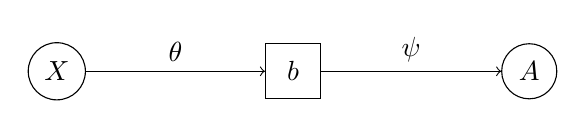
\begin{tikzpicture}[
		roundnode/.style={circle, draw=black, minimum size=7mm},
		squarednode/.style={rectangle, draw=black, minimum size=7mm}
		]
		% nodes
		\node[roundnode] (X) at (0, 0) {$X$};
		\node[squarednode] (b) at (3, 0) {$b$};
		\node[roundnode] (A) at (6, 0) {$A$};
		
		% arrows
		\draw[->] (X.east) -- node[above] {$\theta$} (b.west);
		\draw[->] (b.east) -- node[above] {$\psi$}(A.west);
	\end{tikzpicture}
	\caption{The feature-first block model (FFBM)}
	\label{fig:ffbm}
\end{figure}

Once the block memberships $b$ have been generated, we then draw the graph $A$ from the microcanonical DC-SBM (equation \ref{eqn:A-generation}) with additional parameters encapsulated by $\psi = \{\psi_e, \psi_k\}$.
%
\begin{equation}
	A \sim \textrm{DC-SBM}_{\textrm{MC}} (b, \psi_e, \psi_k)
	\label{eqn:A-generation}
\end{equation}


\subsection{Prior selection}

Before performing any inference, we must specify priors on $\theta$ and $\psi$. For $\theta$ it seems sensible to choose a Gaussian prior, with zero mean and variance matrix $\sigma^2_\theta I$ such that each element of $\theta$ is independent and distributed like $\sim \Gaussian(0, \sigma_\theta^2)$. In vector form, the prior for $\theta$ is therefore:
%
\begin{equation}
	p(\theta) = \Gaussian \left( \theta ; 0, \sigma_\theta^2 I \right)
	\label{eqn:theta-prior}
\end{equation}
%
In our model, the block memberships vector $b$ is an intermediate latent variable and so we are not free to choose a prior for it. Nevertheless, as far as inference on the right-hand-side of figure \ref{fig:ffbm}, we regard $p(b | X)$ as a pseudo-prior on $b$. We can show (appendix \ref{appdx:b|x}) that our choice of prior for $p(\theta)$ in equation \ref{eqn:theta-prior} leads to a uniform $p(b | X)$ in equation \ref{eqn:b-pseudo-prior}.
%
\begin{equation}
	p(b | X) = \int p(b | X, \theta) p(\theta) d\theta = B^{-N}
	\label{eqn:b-pseudo-prior}
\end{equation}
%
This is an enormously important simplification as evaluating $p(b | X)$ does not require an expensive Monte-Carlo integration over the $\theta$-domain nor does it require the exact value of $X$. \citet{Peixoto-Bayesian-Microcanonical} proposes careful choices for the additional microcanonical SBM parameters $\psi$ which we adopt. Peixoto's idea is to write the joint prior on $(b, e, k)$ as a product of conditionals $p(b, e, k) = p(b) p(e | b) p(k | e, b)= p(b) p(\psi | b)$. For our purposes we must insert a conditioning on $X$, to form our pseudo-prior for $b$ and $\psi$, to give equation \ref{eqn:joint-pseudo-prior}.
%
\begin{equation}
	p(b, \psi | X) = p(b | X) p(\psi | b, X) = p(b | X) p(\psi | b)
	\label{eqn:joint-pseudo-prior}
\end{equation}
%
Where we leverage the fact $(\psi \indep X) | b$. We then borrow the priors proposed by \citet{Peixoto-Bayesian-Microcanonical} for $p(\psi | b)$ to complete our model. Please refer to appendix \ref{appdx:sbm} for the exact form of $p(\psi | b)$. All that concerns the main argument is we have a computable form.


\section{Inference}
\label{sec:inference}

Now that we have defined the FFBM, we wish to leverage it to perform inference. Suppose we are presented with a vertex-labelled graph $(A, X)$; the goal is to draw samples for $\theta$ according to the posterior given the observed data:
%
\begin{equation}
	\label{eqn:theta-target}
	\theta^{(t)} \sim p(\theta | A, X)
\end{equation}
%
However, generating these samples is not easily done in practice. We therefore propose an iterative approach. We first draw samples $b^{(t)}$ from the block membership posterior (equation \ref{eqn:b-samples}) and then use each $b^{(t)}$ to draw samples for $\theta$ as in equation \ref{eqn:theta-samples}. 
%
\begin{align}
	b^{(t)} &\sim p \Big( b | A, X \Big)  \label{eqn:b-samples}\\
	\theta^{(t)} &\sim p\Big(\theta | X, b^{(t)} \Big) \label{eqn:theta-samples}
\end{align}
%
Both of these sampling steps can be implemented with a Markov Chain through the Metropolis-Hastings algorithm \cite{hastings-alg}. We just need to define a proposal distribution $q(x, x')$ for proposing a move $x \rightarrow x'$ and be able to evaluate an un-normalised form of the target distribution, denoted $\pi(\cdot)$, point-wise. The proposed move is then accepted with probability $\alpha$ (equation \ref{eqn:mh-accept}) else it is rejected and we stay at $x$.
%
\begin{equation}
	\alpha(x, x') = \min \left( \frac{\pi(x') q(x', x)}{\pi(x) q(x, x')} , 1 \right)
	\label{eqn:mh-accept}
\end{equation}
%
This accept-reject step ensures the resulting Markov Chain is in detailed balance with the target distribution $\pi(\cdot)$. What we propose in equations \ref{eqn:b-samples} and \ref{eqn:theta-samples} is therefore implemented through a 2-level Markov chain. The resulting samples for $\theta^{(t)}$ are unbiased in the sense that the expectation of their distribution is the posterior we are targetting:
%
\begin{equation}
\Expect_{b^{(t)}} \left[p \left( \theta | X, b^{(t)} \right) \right] = \sum_{b \in [B]^N} p(\theta | X, b) p(b | A, X) = \sum_{b \in [B]^N} p(\theta, b | A, X) = p(\theta | A, X)
\label{eqn:theta-unbiased}
\end{equation}
%
This is an example of a pseudo-marginal approach. Indeed, \citet{pseudo-marginal} show that the unbiased result in equation \ref{eqn:theta-unbiased} is sufficient to prove that for large enough $t$, $\theta^{(t)} \sim \Expect_{b^{(i)}} \left[ p(\theta | X, b^{(t)})\right] = p(\theta 
| A, X)$ which is exactly the distribution we are targetting (equation \ref{eqn:theta-target}).
%
\begin{figure}[!h]
	\centering

	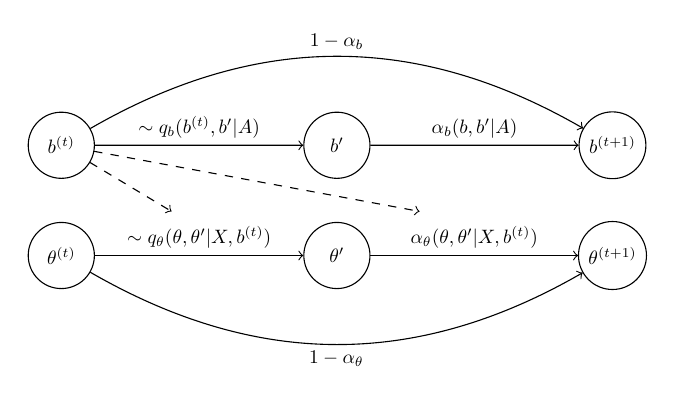
\begin{tikzpicture}[
		scale=0.7, every node/.style={transform shape},
		roundnode/.style={circle, draw=black, minimum size=12mm},
		squarednode/.style={rectangle, draw=black, minimum size=12mm}
		]
		% nodes
		\node[roundnode] (b0) at (0, 2) {$b^{(t)}$};
		\node[roundnode] (b1) at (5, 2) {$b'$};
		\node[roundnode] (b2) at (10, 2) {$b^{(t+1)}$};
		\node[roundnode] (t0) at (0, 0) {$\theta^{(t)}$};
		\node[roundnode] (t1) at (5, 0) {$\theta'$};
		\node[roundnode] (t2) at (10, 0) {$\theta^{(t+1)}$};
		
		% arrows
		\draw[->] (b0) to node[above] {$\sim q_b(b^{(t)}, b' | A)$} (b1);
		\draw[->] (b1) to node[above] {$\alpha_b (b, b' | A)$} (b2);
		\draw[->] (b0) [out=30, in=150] to node[above] {$1-\alpha_b$} (b2);
		
		\draw[->] (t0) to node[above] {$\sim q_\theta(\theta, \theta' | X, b^{(t)})$} (t1);
		\draw[->] (t1) to node[above] {$\alpha_\theta (\theta, \theta' | X, b^{(t)})$} (t2);
		\draw[->] (t0) [out=-30, in=-150] to node[below] {$1-\alpha_\theta$} (t2);
		
		\draw[dashed, ->] (b0) to (2, 0.8);
		\draw[dashed, ->] (b0) to (6.5, 0.8);
		
	\end{tikzpicture}
	\caption{Sampling sequence}
	\label{fig:samp-sequence}
\end{figure}

The reason we split the Markov chain into two stages is because the summation over all latent states $b \in [B]^N$ required to directly compute the likelihood $p(A| X, \theta) = \sum_{b \in [B]^N} p(A | b) P(b | X, \theta)$ is intractable -- $O(B^N)$. Figure \ref{fig:samp-sequence} shows an overview of the proposed method. We have introduced subscripts and conditionings to make explicit what variables each step utilises. We note the power of the simplification given by equation \ref{eqn:b-pseudo-prior}. As $p(b| X)$ does not depend on the exact value of X, we do not need to know the value of $X$ to perform the sampling on $b$. Conversely, for the $\theta^{(t)}$ samples, we use only $b^{(t)}$ but not $A$ as $(\theta \indep A) | b$.

\FloatBarrier

\subsection{Sampling block memberships}

\citet{Peixoto-MCMC} proposes a Monte Carlo method which we will base our approach on. It relies on writing the posterior in the following form:
%
\begin{equation}
	p(b | A, X) \propto p(A | b, X) \cdot p(b | X) = \pi_b(b)
\end{equation}
%
Now $\pi_b(\cdot)$ is the un-normalised density we wish to sample from for the $b$-chain. In other words, we wish to construct a Markov chain that has $\pi_b(\cdot)$ as its invariant distribution. We can break $\pi_b$ down as follows:
%
\begin{equation}
	\pi_b(b) = p(b|X) \sum_{\psi} \nolimits p(A , \psi | b, X) \\
	= p(b|X) p(A, \psi^* | b, X) \\
	= p(A | b, \psi^*) \cdot p(\psi^* | b) \cdot p(b | X)
\end{equation}
%
Since we are using the microcanonical SBM formulation, there is only one value of $\psi$ that is compatible with the given $(A, b)$ pair (given in equation \ref{eqn:sbm-constraints}). We denote this value $\psi^* = \{\psi_k^*, \psi_e^*\}$. Therefore, the summation over all $\psi$ reduces to just the single $\psi^*$ term; this is the power of the microcanonical formulation. We also define the microcanonical entropy of the configuration as.
%
\begin{equation}
	S(b) = - \log \pi_b(b) = - \Big( \log p(A | b, \psi^*) + \log p(\psi^*, b | X) \Big)
	\label{eqn:dl-form}
\end{equation}
%
This entropy can equally be thought of as the description length of the graph. The exact form of the proposal $q_b$ is explored thoroughly by \citet{Peixoto-MCMC} and not repeated here. There is a widely used library for Python made available under LGPL called \verb*|graph-tool| \cite{peixoto_graph-tool_2014}, which implements this algorithm. The only modification we make is in the block membership prior $p(b)$ which we replace with $p(b|X)=B^{-N}$, which cancels out in the MH accept-reject step as it is independent of $b$.

\subsection{Sampling feature-to-block generator parameters}

The invariant distribution we wish to target for the $\theta$ samples is the posterior of $\theta$ given the values of the pair $(X, b)$. We write this as follows:
%
\begin{equation}
	\pi_\theta(\theta) \propto p(\theta | X, b) \propto p(b | X, \theta) p(\theta) \propto \pi_\theta (\theta) \propto  \exp \left( - U(\theta) \right)
\end{equation}
%
Where we have introduced $U(\theta)$ equal to the negative log posterior. We define $y_{ij} \coloneqq \one \left\{ b_i = j \right\}$ and $a_{ij} \coloneqq \phi_j(x_i; \theta)$. Discarding constant terms, we can write $U(\theta)$ as in equation \ref{eqn:U-form} (refer to appendix \ref{appdx:form-U} for the derivation).
%
\begin{equation}
	U(\theta) = \left( \sum_{i=1}^{N} \sum_{j=1}^{B} y_{ij} \log \frac{1}{a_{ij}} \right)
	+ \frac{1}{2\sigma_\theta^2} ||\theta||^2 = N \cdot \Lcal(\theta) + \frac{1}{2\sigma_\theta^2} ||\theta||^2
	\label{eqn:U-form}
\end{equation}
%
$U(\theta)$ in equation \ref{eqn:U-form} appears a typical objective function for neural network training. The first term is introduced by the likelihood. We collect it into $N \cdot \Lcal(\theta)$, which is the cross-entropy between the graph-predicted and feature-predicted block memberships summed over all vertices. The second term of equation \ref{eqn:U-form} -- introduced by the prior -- brings a form of regularisation, guarding against over-fitting. Different to traditional applications, our goal is not to find the minimiser of $U(\theta)$ but to draw samples from the posterior $\pi_\theta(\cdot) \propto \exp(-U(\cdot))$. We can use $\nabla U$ as a useful heuristic to bias our proposal towards regions of higher target density. We therefore adopt the Metropolis-adjusted Langevin algorithm (MALA) -- first proposed by \citet{mala-tweedie}. Given the current sample $\theta$, we generate a new sample $\theta'$ according to equation \ref{eqn:theta-update}.
%
\begin{align}
	\theta' &= \theta - h \nabla U(\theta) + \sqrt{2h} \cdot \xi
	\label{eqn:theta-update} \\
	\therefore q_\theta(\theta, \theta') &= \Gaussian \left( \theta' ; \theta - h \nabla U(\theta), 2h I \right)
	\label{eqn:theta-proposal}
\end{align}
%
Where $\xi \sim \Gaussian(0, I)$ and $h$ is a step-size parameter -- which may vary with the sample index (appendix \ref{appdx:step-size} explores this more fully). Without the injected noise term, MALA is equivalent to gradient descent. We require the noise term $\xi$ to fully explore the parameter space. We can write the proposal distribution $q_\theta$ as in equation \ref{eqn:theta-proposal}. The term $\nabla U$ has an easy to compute analytic form (derived in Appendix \ref{appdx:gradu}). By noting that $\theta = \{w_k\}_{k=1}^{B}$, we write the derivative with respect to each $w_k$ as:
%
\begin{equation}
	\frac{\partial U}{\partial w_k} = - \left( \sum_{i=1}^{N} \Big\{ \tilde{x}_i (y_{ik} - a_{ik}) \Big\} - \frac{w_k}{\sigma_\theta^2} \right)
	\label{eqn:U-derivative}
\end{equation}
%
After a proposed move is generated, in typical Metropolis-Hastings fashion we accept the move with probability $\alpha_\theta$, as in equation \ref{eqn:mh-accept}.

\subsection{Sampling sequence}

Up to this point, each $\theta^{(t)}$ update uses its corresponding $b^{(t)}$ sample. This means that the evaluation of $U(\theta)$ and $\nabla U(\theta)$ has high variance. This may lead to longer burn-in for the resulting Markov chain. The only link between $b^{(t)}$ and $\theta^{(t)}$ is in the evaluation of $U(\theta)$ and $\nabla U(\theta)$ which depends only on the matrix $y^{(t)}$ with entries $y_{ij}^{(t)} \coloneqq \one\{b_i^{(t)} = j\}$. We would rather deal with the expectation of each $y_{ij}^{(t)}$:
%
\begin{equation}
	\Expect \left[ y_{ij}^{(t)} \right] = \Expect_{b^{(t)}} \left[ \one(b_{i}^{(t)} = j) \right]
	= p(b_i = j | A, X)
\end{equation}
%
We can obtain an unbiased estimate for this quantity using the set of $b$-samples. However, as with all MCMC methods, we must only uses samples after burn-in and thinning have been applied. We introduce $\Tcal_b$ to denote the retained set of indices for the $b$-samples and $\Tcal_\theta$ similarly for the $\theta$-chain. An in-depth discussion of how these sets are chosen is given in appendix \ref{appdx:burn-in-thinning}. The unbiased estimate for $y_{ij}^{(t)}$ using the restricted sample set $\Tcal_b$ is denoted $\hat{y}_{ij}$ and has form:
%
\begin{equation}
	\hat{y}_{ij} \coloneqq \frac{1}{|\Tcal_b|} \sum_{t \in \Tcal_b} y_{ij}^{(t)} = \frac{1}{|\Tcal_b|} \sum_{t \in \Tcal_b} \one\{b_i^{(t)} = j\}
\end{equation}
%
We choose to feed each $\theta^{(t)}$ update step the same matrix $\hat{y}$ for all $t$ rather than the corresponding $y^{(t)}$. This means we no longer need to run the $b$ and $\theta$ Markov chains concurrently. Instead, we run the $b$-chain to completion and use it to generate $\hat{y}$. This affords us the flexibility to vary the lengths of the $b$ and $\theta$-chains. Furthermore, the changeover from $y^{(t)}$ to $\hat{y}$ reduces the burn-in time for the $\theta$-chain by reducing the variance in our evaluation of $U$ and $\nabla U$. A description of the overall algorithms is given in appendix \ref{appdx:algorithms}.

\subsection{Dimensionality reduction}
\label{sec:dim-reduction}

Once we have the samples $\left\{ \theta^{(t)} \right\} \sim p(\theta | A, X)$, we can compute the empirical mean and standard deviation of each component of $\theta$. Switching back to matrix notation we define $\theta = W$, such that $W_{ij}$ is the weight component for block $i$ and feature $j$, we can define:
%
\begin{equation}
	\hat{\mu}_{ij} \coloneqq \frac{1}{|\Tcal_\theta|} \sum_{t \in \Tcal_\theta} W_{ij}^{(t)} \qquad \textrm{and} \qquad
	\hat{\sigma}_{ij} \coloneqq \frac{1}{|\Tcal_\theta|} \sum_{t \in \Tcal_\theta} \left( W_{ij}^{(t)} - \hat{\mu}_{ij} \right)^2
\end{equation}
%
A simple heuristic to discard the least important features requires specifying a cutoff $c > 0$ and a multiplier $k > 0$. We define the function $\Fcal_i(j)$ as in \ref{eqn:fij} then only keep features with indices $d \in \Dcal'$, where $\Dcal'$ is constructed as in equation \ref{eqn:kept-feature-set}.
%
\begin{align}
	\Fcal_i(j) &\coloneqq (\hat{\mu}_{ij} - k \hat{\sigma}_{ij}, \hat{\mu}_{ij} + k \hat{\sigma}_{ij}) \cap (-c, +c)
	\label{eqn:fij} \\
	\Dcal' &\coloneqq \left\{ j \in [D] : \exists i \in [B] \textrm{ s.t. }  \Fcal_i(j) \neq \emptyset \right\}
	\label{eqn:kept-feature-set}
\end{align}
%
Intuitively, this means discarding any feature for which $\hat{\mu}_{ij} \pm k\hat{\sigma}_{ij}$ lies within or spans the null region $(-c, c)$ for all block indices. If we were to use the Laplace approximation for the posterior $p(W_{ij} | A, X) \approx \Gaussian(W_{ij}; \mu_{ij}, \sigma_{ij})$, then this is effectively a hypothesis test on the value of $W_{ij}$ (equation \ref{eqn:hyp-test-discard}). $\Dcal'$ then comprises all features $i$ for which $H_1$ is accepted at least once for some $j \in [B]$.
%
\begin{equation}
	H_0: |\mu_{ij}| \leq c \qquad
	H_1: |\mu_{ij}| > c
	\label{eqn:hyp-test-discard}
\end{equation}
%
The multiplier $k$ determines the degree of significance of the result. However, as the Laplace approximation is not exact we will only treat this dimensionality reduction method as a useful heuristic and not an exact method. Conversely, we could fix $k=k_0$ and the dimension of our reduced feature set $|\Dcal'|=D'$. We would then like to find the largest value of $c$ such that $|\Dcal'|=D'$ given $k=k_0$. This is summarised in equation \ref{eqn:c-star}. This approach is often preferred as it fixes the number of reduced dimensions.
%
\begin{equation}
	c^* = \argmax_{c>0} (c : |\Dcal'| = D', k=k_0)
	\label{eqn:c-star}
\end{equation}

\section{Experiments}
\label{sec:experiments}

We apply the outlined methods to a variety of datasets:

\begin{itemize}
	\item \textbf{Political books} \cite{polbooks} ($N=105, E=441, D=3$) -- network of Amazon political book sales, published close to the 2004 presidential election. Two books are connected if they were frequently co-purchased. Vertex features encode the political affiliation of the author (liberal, conservative, or neutral).
	\item \textbf{Primary school dynamic contacts} \cite{schools} ($N=238, E=5539, D=13$) -- network of face-to-face contacts amongst students and teachers at a primary school in Lyon, France. Vertex features include class membership (one of 10 values: 1A-5B), gender (male, female) and teacher status encoded as an 11th school-class. We choose to analyse just the second day of results.
	\item \textbf{Facebook egonet} \cite{fb-snap} ($N=747, E=30025, D=480$) -- an assortment of Facebook users' friends lists. Vertex features are fully anonymised and encode information about each user's education history, languages spoken, gender, home-town, birthday etc. We focus on the egonet with id 1912.
\end{itemize}
%
We first require metrics to assess model performance. We define the average
description length per entity (nodes and edges) $\bar{S}_e$ as a suitable metric to gauge the SBM fit:
%
\begin{equation}
	\bar{S}_e \coloneqq \frac{1}{(N+E) |\Tcal_b|} \sum_{t\in \Tcal_b} S \left( b^{(t)} \right).
	\label{eqn:mean-dl}
\end{equation}

Next, to assess the performance of the feature-to-block predictor, 
we randomly partition the vertex set $[N]$ into training and test sets: $\Gcal_0$ and $\Gcal_1$.
The $b$-chain is run using the whole network but we only use vertices $v \in \Gcal_0$ to train the $\theta$-chain. As $|\Gcal_0| \neq |\Gcal_1|$ in general, we use the average cross-entropy loss 
over each set to gauge fit,
%
\begin{equation}
	\bar{\Lcal}_\star \coloneqq \frac{1}{|\Tcal_\theta|} \sum_{t \in \Tcal_\theta} \Lcal_\star^{(t)},
	\quad \textrm{where} \quad
	\Lcal_\star^{(t)} \coloneqq \frac{1}{|\Gcal_\star|} \sum_{i \in \Gcal_\star}\sum_{j \in [B]} \hat{y}_{ij} \log \frac{1}{\phi_j \left(x_i; \theta^{(t)} \right)},
	\label{eqn:cross-entropy-loss}
\end{equation}
%
where $\star \in \{0, 1\}$ toggles between the training and test sets.
%
Nevertheless, the cross-entropy loss is a coarse measure of fit. We wish to define a new measure of fit specific to each detected block. Let us define
$
	\Bcal_\star(j) \coloneqq \{i \in \Gcal_\star : \hat{b}_i = j\}
$
where
$ 
	\hat{b}_i \coloneqq \argmax_j \hat{y}_{ij}.
$
Now $\Bcal_\star(j)$ is the set of vertices that have maximum a posteriori probability of belonging to block $j$. We now define the accuracy for block $j$ as,
%
\begin{equation}
	\eta_\star(j) \coloneqq \frac{1}{|\Bcal_\star (j)| \cdot 
	|\Tcal_\theta| } 
	\sum_{i \in \Bcal_\star (j)}  \sum_{t \in \Tcal_\theta}
	\one \left\{\hat{b}_i = \argmax_j \phi_j \left( x_i; \theta^{(t)} \right) \right\}.
	\label{eqn:accuracy}
\end{equation}

This effectively tests whether the feature-to-block and the graph-to-block predictions agree in their largest component. We call this metric, $\eta_\star(j)$, the {\em block-accuracy} for block $j$. It is clearly bounded $0 \leq \eta_\star(j) \leq 1$, with an accuracy of 1 meaning perfect agreement for the vertices in detected block $j$.

Table~\ref{tab:results} summarises the results for each experiment. 
We see that the dimensionality reduction procedure 
brings the training and test losses closer together. This implies that 
the features we keep are indeed correlated with the underlying graphical 
partition and that the approach generalises correctly. The test loss variance is higher than the training loss variance as the test set is smaller and so more susceptible to variability in its construction.
%
The average description length per entity,
$\bar{S}_e$, of the graph, 
has very small variance, suggesting that
the detected communities can be found reliably (to within an arbitrary 
relabelling of blocks).

\paragraph{\textbf{Political books.}}

We choose to partition the network into $B=3$ communities as we only have this many distinct values for political affiliation.
From Figure~\ref{fig:polbooks-null} we see that all 3 blocks have a distinct political affiliation as their largest positive component.  
Furthermore, the training and test losses from Table~\ref{tab:results}  
are very similar and both are low in magnitude. This is strong evidence 
that political affiliation is a very appropriate explanatory 
variable for the overall network structure.
%
However, from Figure~\ref{fig:polbooks-accuracy} we see that block 1 has low accuracy. 
This suggests that detected block 1 is not solely composed of ``neutral" books but also 
contains some ``liberal" and ``conservative" authors. Examining 
Figure~\ref{fig:polbooks-graph}, we see the majority of paths between blocks 2 and 3 go through block 1.
Block 1 is in effect a bridge between the ``conservative'' and ``liberal'' blocks so it is unsurprising that some of these leak into block 1.

\paragraph{\textbf{Primary school.}}

We choose the number of communities $B=10$, in line with the total number of 
school classes. Only the pupils' class memberships (1A-5B) survive
the dimensionality-reduction process (Figure~\ref{fig:school-null});
gender and teacher/student status have been discarded,
meaning these are poor predictors of overall macro-structure.
%
The vast majority of blocks are composed of a single class. 
However, some blocks have two comparably strong classes as their predictors (e.g. blocks 2 and 5). 
Conversely, some classes are found to extend over two 
detected blocks (class 2B spans blocks 8 and 9) but we do 
not have a feature which explains the division.
%
Figure~\ref{fig:school-accuracy} shows excellent accuracy for the majority of blocks. In fact the only blocks with low accuracy are those that have a school-class span two blocks such that we cannot reliably distinguish between the two. This is more pronounced when we apply hard classification rather than the soft cross-entropy loss. Perhaps there are unobserved features which explain this divide.

\paragraph{\textbf{Facebook egonet.}}

The retained features 
(Figure~\ref{fig:fb-null}) are those that best explain the high-level 
community structure. The majority of these are education related. 
Nevertheless, for $D'=10$ we only have good explanations for some of the detected blocks; several blocks in 
Figure~\ref{fig:fb-null} do not have high-magnitude components. This is further emphasised by the disparate accuracies in Figure~\ref{fig:fb-accuracy}.
%
For a high-dimensional feature-space, it is likely that a particular
feature may uniquely identify a small set of vertices; if these are all in the same block, then the classifier may overfit despite the penalty imposed by the prior. Indeed, we see in
Figure~\ref{fig:fb-null} that the feature birthday-5 has a very high weight as it relates to block 1 – but it is unlikely that birthdays determine graphical structure.
\begin{table}[!ht]
	\centering
	\caption{Results averaged over $n=10$ iterations (mean $\pm$ std. dev.).}
	\label{tab:results}
	\resizebox{\textwidth}{!}{%
		\begin{tabular}{c|ccc|c|cc|ccc}
			Dataset  & $B$ & $D$ & $D'$ & $\bar{S}_e$ & $\bar{\mathcal{L}}_0$ & $\bar{\mathcal{L}}_1$ & $c^*$ & $\bar{\mathcal{L}}_0'$ & $\bar{\mathcal{L}}_1'$  \\ \hline
			Polbooks & 3 & 3 & -- & $2.250 \pm 0.000$ & $0.563 \pm 0.042$ & $0.595 \pm 0.089$ & -- & -- & -- \\
			School & 10 & 13 & 10 & $1.894 \pm 0.004$ & $0.787 \pm 0.127$ & $0.885 \pm 0.129$ & $1.198 \pm 0.249$ & $0.793 \pm 0.132$ & $0.853 \pm 0.132$ \\
			FB egonet & 10  & 480 & 10 & $1.626 \pm 0.003$ & $1.326 \pm 0.043$ & $1.538 \pm 0.069$ & $0.94 \pm 0.019$ & $1.580 \pm 0.150$ & $1.605 \pm 0.106$
		\end{tabular}
	}
\end{table}

\begin{figure}[!ht]
	\centering
	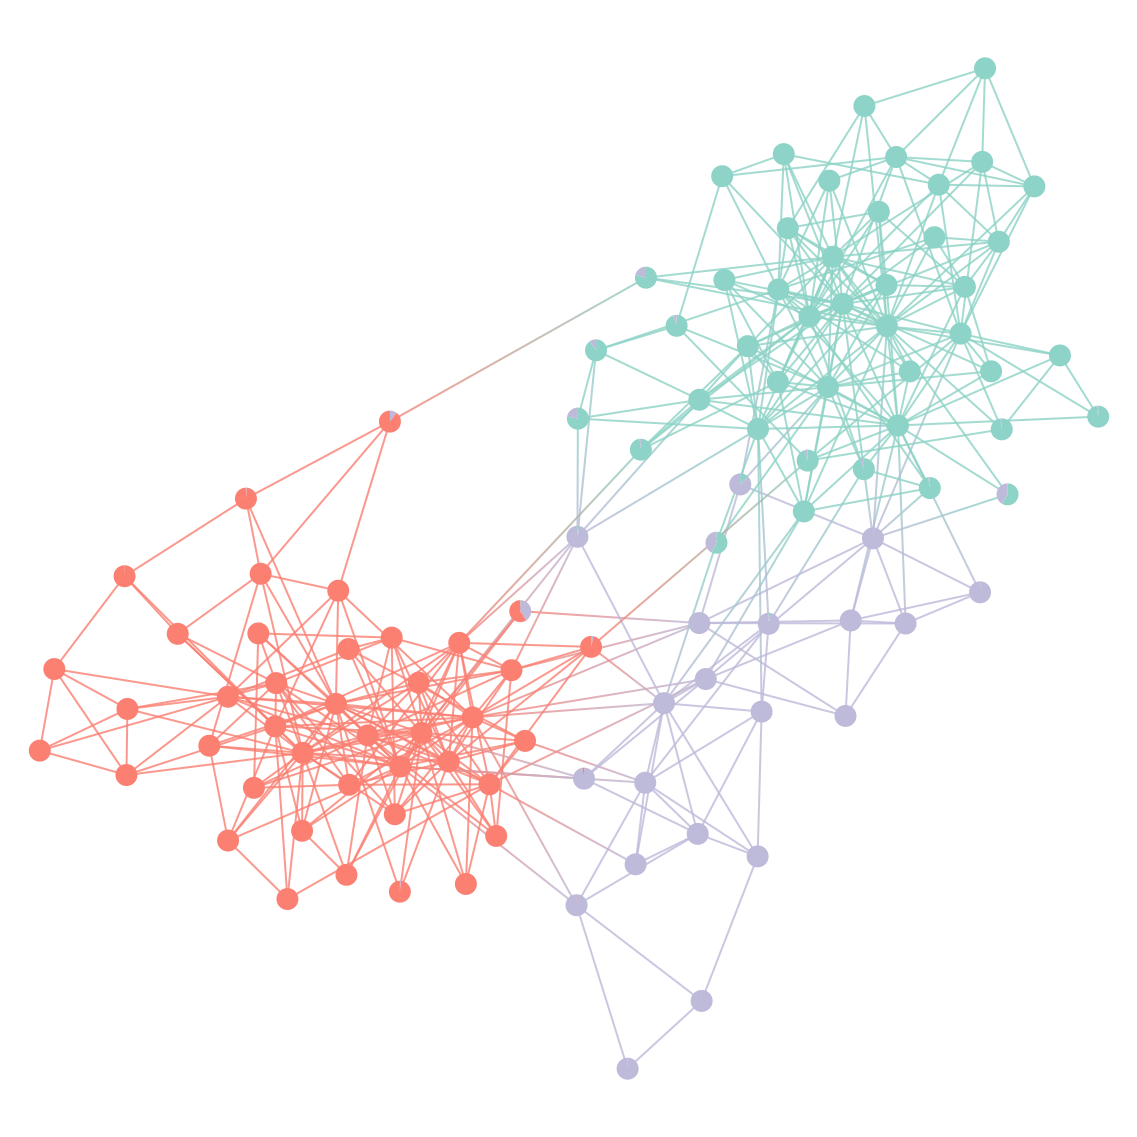
\includegraphics[width=0.28\linewidth]{img/polbooks-graph.png}
	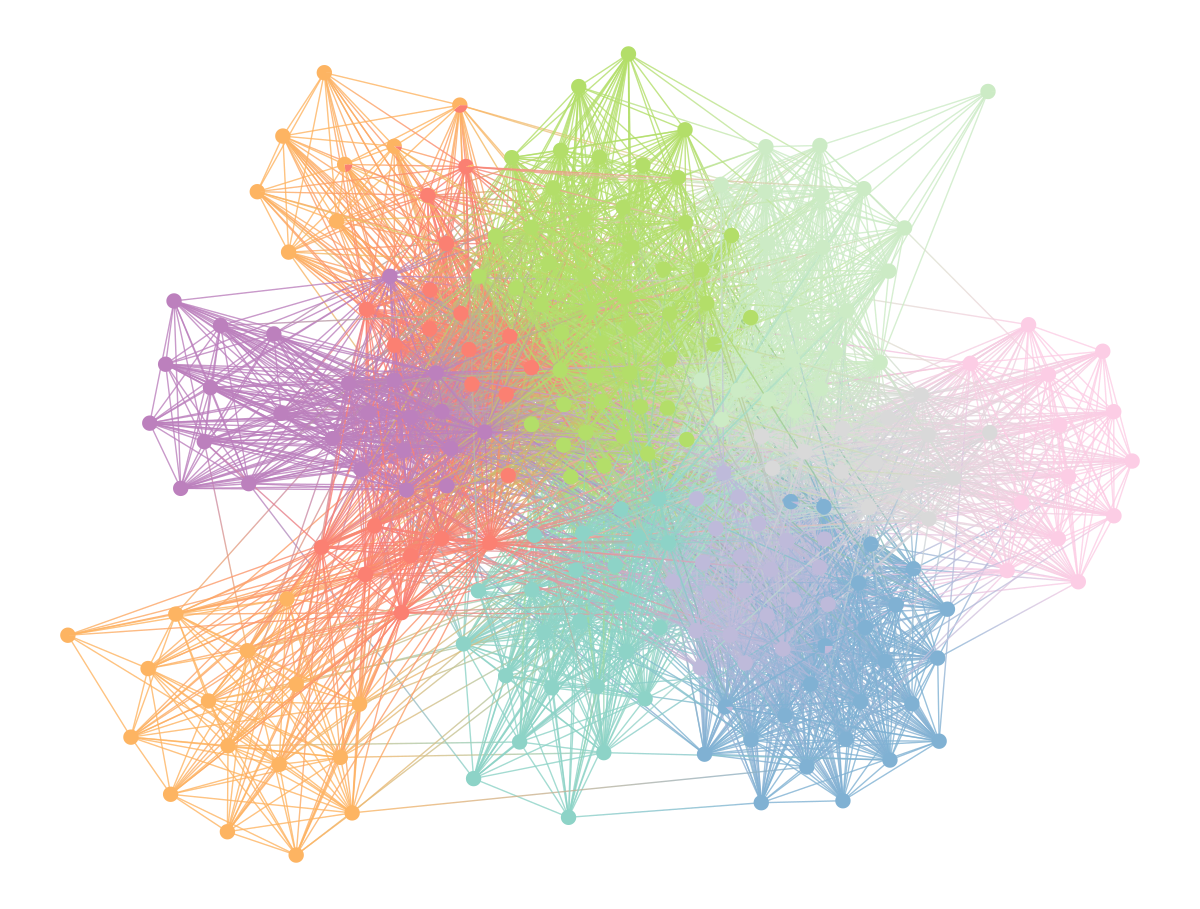
\includegraphics[width=0.28\linewidth]{img/school-graph.png}
	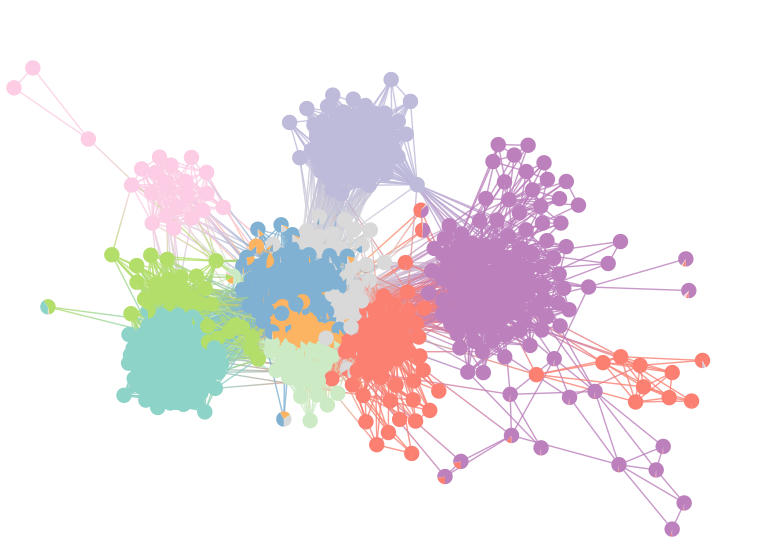
\includegraphics[width=0.28\linewidth]{img/fb-graph.png}
	\caption{Networks laid out and coloured according to inferred block memberships. Left to right: Polbooks, Krebs (2004); Primary School, Stehle et al (2011); Facebook Egonet, Leskovec and Mcauley (2012).}
	\label{fig:graphs-all}
\end{figure}



%\section{Extensions}

The current FFBM formulation can only explain macro-structure and not structure within each detected block. Future work will benefit from extending the FFBM to be hierarchical in nature. Indeed, the SBM has already been extended to a hierarchical form, often called the nested SBM \cite{SBM-hierarchical}.

The necessary modification of the feature-to-block generator is also rather natural. Given the nested SBM, we would have a hierarchy of generators, each generating a block membership at a particular level of the hierarchy. To avoid exponential growth in the number of model parameters, we could apply some form of dimensionality reduction as we descend the layers so that each generator is only given relevant features as input.

\section{Conclusion}
\label{sec:conclusion}

The feature-first block model
(FFBM) is introduced, as a 
new generative model for labelled 
networks with communities.
An efficient MCMC algorithm  
is developed for sampling 
from the posterior distribution of
the relevant parameters in the FFBM;
the main idea is to divide up the graph into 
its most natural partition under the associated
parameter values, and then to determine whether 
the vertex features can accurately explain the partition. 
Through applications on empirical
network data, this approach 
is demonstrated to be effective at extracting and describing 
the most natural communities in a labelled network. 
Nevertheless, it
can only currently explain the structure at the macroscopic
scale. Future work will benefit from extending 
the FFBM to a further hierarchical model,
so that
the structure of the network 
can be explained at all scales of interest.




\clearpage
\begin{ack}
	
	\textit{Unsure what to put in this section}
	
	Use unnumbered first level headings for the acknowledgments. All acknowledgments
	go at the end of the paper before the list of references. Moreover, you are required to declare
	funding (financial activities supporting the submitted work) and competing interests (related financial activities outside the submitted work).
	More information about this disclosure can be found at: \url{https://neurips.cc/Conferences/2021/PaperInformation/FundingDisclosure}.
	
	Do {\bf not} include this section in the anonymized submission, only in the final paper. You can use the \texttt{ack} environment provided in the style file to automatically hide this section in the anonymized submission.
\end{ack}

%references
\bibliography{sources.bib}

\clearpage
\section*{Checklist}

%%% BEGIN INSTRUCTIONS %%%
The checklist follows the references.  Please
read the checklist guidelines carefully for information on how to answer these
questions.  For each question, change the default \answerTODO{} to \answerYes{},
\answerNo{}, or \answerNA{}.  You are strongly encouraged to include a {\bf
	justification to your answer}, either by referencing the appropriate section of
your paper or providing a brief inline description.  For example:
\begin{itemize}
	\item Did you include the license to the code and datasets? \answerYes{See Section gen-inst.}
	\item Did you include the license to the code and datasets? \answerNo{The code and the data are proprietary.}
	\item Did you include the license to the code and datasets? \answerNA{}
\end{itemize}
Please do not modify the questions and only use the provided macros for your
answers.  Note that the Checklist section does not count towards the page
limit.  In your paper, please delete this instructions block and only keep the
Checklist section heading above along with the questions/answers below.
%%% END INSTRUCTIONS %%%

\begin{enumerate}
	
	\item For all authors...
	\begin{enumerate}
		\item Do the main claims made in the abstract and introduction accurately reflect the paper's contributions and scope?
		\answerYes{}
		\item Did you describe the limitations of your work?
		\answerYes{See section conclusion}
		\item Did you discuss any potential negative societal impacts of your work?
		\answerTODO{}
		\item Have you read the ethics review guidelines and ensured that your paper conforms to them?
		\answerTODO{}
	\end{enumerate}
	
	\item If you are including theoretical results...
	\begin{enumerate}
		\item Did you state the full set of assumptions of all theoretical results?
		\answerYes{See section inference}
		\item Did you include complete proofs of all theoretical results?
		\answerYes{See section inference}
	\end{enumerate}
	
	\item If you ran experiments...
	\begin{enumerate}
		\item Did you include the code, data, and instructions needed to reproduce the main experimental results (either in the supplemental material or as a URL)?
		\answerTODO{}
		\item Did you specify all the training details (e.g., data splits, hyperparameters, how they were chosen)?
		\answerTODO{}
		\item Did you report error bars (e.g., with respect to the random seed after running experiments multiple times)?
		\answerTODO{}
		\item Did you include the total amount of compute and the type of resources used (e.g., type of GPUs, internal cluster, or cloud provider)?
		\answerTODO{}
	\end{enumerate}
	
	\item If you are using existing assets (e.g., code, data, models) or curating/releasing new assets...
	\begin{enumerate}
		\item If your work uses existing assets, did you cite the creators?
		\answerTODO{}
		\item Did you mention the license of the assets?
		\answerTODO{}
		\item Did you include any new assets either in the supplemental material or as a URL?
		\answerTODO{}
		\item Did you discuss whether and how consent was obtained from people whose data you're using/curating?
		\answerTODO{}
		\item Did you discuss whether the data you are using/curating contains personally identifiable information or offensive content?
		\answerTODO{}
	\end{enumerate}
	
	\item If you used crowdsourcing or conducted research with human subjects...
	\begin{enumerate}
		\item Did you include the full text of instructions given to participants and screenshots, if applicable?
		\answerNA{}
		\item Did you describe any potential participant risks, with links to Institutional Review Board (IRB) approvals, if applicable?
		\answerNA{}
		\item Did you include the estimated hourly wage paid to participants and the total amount spent on participant compensation?
		\answerNA{}
	\end{enumerate}
	
\end{enumerate}

\clearpage
\appendix

\section{Appendix}

\subsection{SBM prior choice explanation}
\label{appdx:prior}

We have borrowed the priors proposed by \citet{Peixoto-Bayesian-Microcanonical} for $p(\psi | b)$. These, are repeated here for reference:
%
\begin{equation}
	p(\psi_e=e, \psi_k=k | b) = p(e | b) p(\psi_k | e, b) = \left[ \specialchoose{ \specialchoose{B}{2} }{ E} \right]^{-1} 
	\cdot \left[ \prod_r \frac{\prod_j \eta_j^r !}{n_r! q(e_r, n_r)} \right]
\end{equation}
%
Where $\specialchoose{n}{m}$ is shorthand for $\binom{n+m-1}{m} = \frac{(n+m-1)!}{(n-1)!(m)!}$ which can be thought of as the total number of distinct histograms with $n$ bins under the constraint they sum to $m$. $E = \frac{1}{2} \sum_{r,s} e_{rs}$ is the total number of edges in the graph. Importantly, $E$ is not allowed to vary and so $p(e|b)$ is uniform with respect to $e$. The variable $\eta_j^r$ is introduced to denote the number of vertices in block $r$ that have degree $j$. Formally, $\eta_j^r \coloneqq \sum_{i} \one\left\{b_i = r \right\} \one \left\{k_i = j \right\}$. Furthermore, $q(m, n)$ is the number of different histograms with at most $n$ non-zero bins that sum to $m$. $q(m, n)$ is related to but different from $\specialchoose{n}{m}$. Lastly, $e_r \coloneqq \sum_{s} e_{rs}$ is the total number of half edges in block r and $n_r \coloneqq \sum_{i} \one\{b_i = r\}$ is the number of vertices assigned to block $r$. 

These were chosen carefully by \citet{Peixoto-Bayesian-Microcanonical} to more closely match the structure of empirical networks than simple uniform priors. We do not repeat his arguments here.

\subsection{Derivation of conditional block distribution given feature matrix}
\label{appdx:b|x}

We wish to determine the form of $p(b| X)$. This can be done by integrating over the joint probability with respect to $\theta$.
%
\begin{align*}
	p(b | X) &= \int p(b , \theta| X, \theta) d\theta = \int p(b | X, \theta) p(\theta | X) d\theta \\
	&=\int p(b | X, \theta) p(\theta) d\theta = \int \prod_{i \in [N] } \phi_{b_i}(x_i; \theta) p(\theta) d\theta \\
	&= \prod_{i \in [N]} \int \frac{\exp(w_{b_i}^T \tilde{x}_i) \prod_{j \in [B]} \Gaussian(w_j; 0, \sigma_\theta^2 I)}{\sum_{k \in [B]} \exp(w_{k}^T \tilde{x}_i)} dw_{1:B}
\end{align*}
%
We note that $b_i \in [B]$ and so the integral's value is unchanged with respect to $b_i$. The integrand has the same form no matter which value $b_i$ takes as the prior is the same for each $w_j$. As such the integral can only be a function of at most $\tilde{x}_i$ and $\sigma_\theta^2$ as it is symmetric with respect to $b_i$ and all the various $w_j$ are integrated out as they are dummy variables. Therefore, denoting the integral by the (unknown) function $f(\tilde{x}_i, \sigma_\theta^2)$, we write $p(b| X)$ as follows:
%
\begin{align*}
	p(b | X) &= \prod_{i=1}^{N} f(\tilde{x}_i, \sigma_\theta^2) = \textrm{const w.r.t } b = c
\end{align*}
%
As this is a constant with respect to $b$ we conclude that $p(b | X)$ must be a uniform distribution. $\nicefrac{1}{c}$ is simply the size of the set of values that $b$ can take. We know $b_i \in [B]$. Therefore, $b \in [B]^N$ and $|[B]^N| = B^N = \nicefrac{1}{c}$. Putting this all together we conclude that:
%
\begin{equation}
	p(b | X) = B^{-N}
\end{equation}

\subsection{Derivation of U form}
\label{appdx:form-U}

The invariant distribution we wish to target for the $\theta$ samples is the posterior of $\theta$ given the values of the pair $(X, b)$. We write this as follows:
%
\begin{align}
	\pi_\theta(\theta) &\propto p(\theta | X, b) \propto p(b | X, \theta) p(\theta) \propto  \exp \left( - U(\theta) \right) \\
	\therefore U(\theta) &= - \left( \log p(b | X, \theta) + \log p(\theta) \right) + \textrm{const}
\end{align}
%
Where we have introduced $U(\theta)$ equal to the negative log posterior. Each of the constituent terms of $U(\theta)$ are easily computed (equation \ref{eqn:U-constituent-terms}) by defining $y_{ij} \coloneqq \one \left\{ b_i = j \right\}$ and $a_{ij} \coloneqq \phi_j(x_i; \theta)$.
%
\begin{equation}
	\log p(b | X, \theta) = \sum_{i \in [N]} \sum_{j \in [B]} y_{ij} \log a_{ij}  \quad \textrm{and} \quad
	\log p(\theta) = -\frac{(D+1)(B)}{2} \log 2\pi - \frac{1}{2 \sigma_\theta^2} || \theta ||^2
	\label{eqn:U-constituent-terms}
\end{equation}
%
Discarding constant terms, we write $U(\theta)$ as in equation \ref{eqn:U-form-appdx-0}. Note that $||\theta||^2 = \sum_{i} \theta_{i}^2 = \sum_{j=1}^{B} ||w_j||^2$ is the Euclidean norm of the vector of parameters $\theta$.
%
\begin{equation}
	U(\theta) = \left( \sum_{i=1}^{N} \sum_{j=1}^{B} y_{ij} \log \frac{1}{a_{ij}} \right)
	+ \frac{1}{2\sigma_\theta^2} ||\theta||^2 = N \cdot \Lcal(\theta) + \frac{1}{2\sigma_\theta^2} ||\theta||^2
	\label{eqn:U-form-appdx-0}
\end{equation}
%

\subsection{Derivation of U gradient with respect to feature parameters}
\label{appdx:gradu}
The goal is to determine $\nabla U(\theta)$, the gradient of the negative log posterior with respect to the parameters. We repeat the form of $U(\theta)$ in equation \ref{eqn:U-form-appdx}.
%
\begin{equation}
	U(\theta) = \left( \sum_{i \in [N]} \sum_{j \in [B]} y_{ij} \log \frac{1}{a_{ij}} \right)
	+ \frac{1}{2\sigma_\theta^2} ||\theta||^2
	\label{eqn:U-form-appdx}
\end{equation}
%
Where $y_{ij}$ is independent of $\theta$ and $a_{ij}$ is the output from the softmax layer, with form as given in equation \ref{eqn:a-ij}.
%
\begin{equation}
	a_{ij} \coloneqq \phi_{j} (x_i; \theta) = \frac{\exp(w_j^T \tilde{x}_i)}{\sum_{r \in [B]} \exp(w_r^T \tilde{x}_i)}
	\label{eqn:a-ij} 
\end{equation}
%
We note that $\theta = \{w_k\}_{k=1}^B$, and as such we can write this in vector form $\theta = \left[w_1^T, w_2^T \dots w_B^T  \right]^T$. Therefore, $\nabla U(\theta) = \left[\nicefrac{\partial U}{\partial w_1}^T,\nicefrac{\partial U}{\partial w_2}^T \dots \nicefrac{\partial U}{\partial w_B}^T  \right]^T$; to compute $\nabla U(\theta)$ it suffices to find the form of $\nicefrac{\partial U}{\partial w_k}$ with respect to a general $k$.

To this end, we must first find partial derivatives of $a_{ij}$ and $||\theta||$ with respect to $w_k$. Starting with $a_{ij}$:
%
\begin{align}
	\frac{\partial a_{ij}}{\partial w_k} &= \frac
	{\tilde{x}_i \exp(w_j^T \tilde{x}_i) \delta_{jk} \cdot \sum_{r \in [B]} \exp(w_r^T \tilde{x}_i) 
		- 
		\exp(w_j^T \tilde{x}_i) \cdot \tilde{x}_i \exp(w_k^T \tilde{x}_i)}
	{\left( \sum_{r \in [B]} \exp(w_r^T \tilde{x}_i) \right)^2} \nonumber \\
	&= \tilde{x}_i \left( a_{ij} \delta_{jk} - a_{ij}a_{ik} \right) 
\end{align}
%
Where $\delta_{jk} \coloneqq \one \left\{ j = k \right\}$. Now moving onto the derivative of $||\theta||^2$:
%
\begin{equation}
	\frac{ \partial}{\partial w_k} ||\theta||^2 = \frac{\partial}{\partial w_k} \left( \sum_{r \in [B]} ||w_r||^2 \right) = 2w_k
\end{equation}
%
We are ready to put this all together, to find the partial derivative of $U(\theta)$ with respect to each $w_k$:
\begin{align}
	\frac{\partial U}{\partial w_k} &= 
	\sum_{i=1}^{N} \sum_{j=1}^{B} y_{ij} 
	\left( \frac{-\tilde{x}_i}{a_{ij}} \left( a_{ij} \delta_{jk} - a_{ij} a_{ik} \right) \right)
	+ \frac{w_k}{\sigma_\theta^2} \nonumber \\
	&=  - \left( \sum_{i=1}^{N} \tilde{x}_i \left( y_{ik} - a_{ik} \sum_{j=1}^{B} y_{ij} \right)
	- \frac{w_k}{\sigma_\theta^2} \right) \nonumber \\
	&= - \left( \sum_{i=1}^{N} \Big\{ \tilde{x}_i (y_{ik} - a_{ik}) \Big\} - \frac{w_k}{\sigma_\theta^2} \right)
\end{align}
%
This is the required result. This form can be computed efficiently through matrix operations. The only property of $y_{ij}$ we have used in the derivation is the sum-to-one constraint $\sum_{j=1}^{B} y_{ij} = 1$ for all $i$.

\subsection{Choosing the MALA step-size}
\label{appdx:step-size}

For sampling from the $\theta$-chain of the block membership generator parameters, we employed the Metropolis Adjusted Langevin Algorithm (MALA). At iteration $t$, the proposed sample is generated by:
%
\begin{equation}
	\theta' = \theta^{(t)} - h_t \nabla U(\theta^{(t)}) + \sqrt{2h_t} \cdot \xi
\end{equation}
%
There are two competing objectives when choosing the step-size $h_t$. On the one hand, we want the step-size to be large so that we arrive at a high density region quickly. However, too large a step-size will lead to a lower acceptance ratio and thus inefficient sampling. A solution to this problem would be to slowly decrease the step-size with $t$ - often called simulated annealing. Therefore, we still have a short burn-in time but will not bounce around the mode for large $t$. As well as the trivial constraint for $h_t$ to be strictly positive, we introduce two further constraints as outlined by \citet{Bayesian-SGLD}:
%
\begin{equation}
	\sum_{t=1}^{\infty} h_t = \infty \qquad \textrm{and} \qquad
	\sum_{t=1}^{\infty} h_t^2 < \infty
	\label{eqn:h-constraints}
\end{equation}
%
The first constraint ensures that we have cover sufficient distance to arrive at any arbitrary point in our domain, no matter the starting point. The second constraint ensures that once we converge to the mode rather than simply bouncing around it. \citet{Bayesian-SGLD} propose the following form for a polynomially decaying step-size which we adopt:
%
\begin{equation}
	h_t = \alpha(\beta + t)^{-\gamma}
\end{equation}
%
Where $\alpha, \beta, \gamma$ are hyper-parameters to be chosen. We require $\alpha,\beta > 0$ and $\gamma \in (0.5, 1]$ to satisfy equation \ref{eqn:h-constraints}. To reduce the number of hyperparameters we set these to have values given by the equations \ref{eqn:step-size-params}.
%
\begin{equation}
	\alpha = \frac{250 \cdot s}{N} \qquad \beta = 1000 \qquad \gamma = 0.8
	\label{eqn:step-size-params}
\end{equation}
%
Where $N$ is the number of data-points we are considering and now $s$ is the only free variable which we call the step-size scaling. For approximate methods, we can choose to bypass the MH accept-reject entirely to speed up computation. If this is done, the algorithm is instead called stochastic gradient Langevin diffusion (SGLD) \cite{Bayesian-SGLD}. This speeds up computation at the expense of exactness of the method.

\subsection{Burn-in and thinning}
\label{appdx:burn-in-thinning}

As with any MCMC method, we must deal with the issues presented by burn-in and thinning. We have introduced the notation $\Tcal_b$ and $\Tcal_\theta$ to denote the set of samples we keep from the $b$ and $\theta$ chains respectively. Note that we generate $T_b$ and $T_\theta$ samples total. The burn-in period refers to the time taken for the Markov Chain to converge to the stationary distribution. Sample thinning is necessary to ensure that neighbouring samples satisfy independence. However, as we do not leverage the independence property this is less important in our analysis. We can write the general set $\Tcal_\star$ as:
%
\begin{equation}
	\Tcal_\star = \{T_\star \kappa_\star + i \lambda_\star :  
	0 \leq i \leq \lfloor T_\star(1 - \kappa_\star) / \lambda_\star \rfloor \}
\end{equation}
%
Where the parameter $\kappa_\star \in (0, 1)$ controls our burn-in and $\lambda_\star$ controls our thinning. $\kappa_\star$ can be determined by plotting the log-target (either $S(b^{(t)})$ or $U(\theta^{(t)})$ with respect to the epoch $t$. $\kappa_\star$ is then chosen to encompass the region where the log-target has roughly equilibrated. As we do not leverage sample independence $\lambda_\star$ can be chosen less rigorously. We often just use $\lambda_b=5$ and $\lambda_\theta = 10$.

\subsection{Initializing the b-chain}

For the purposes of our model (the FFBM), the number of blocks $B$ is a constant which must be specified by the data scientist. We could however, allow our choice of $B$ to be influenced by the observed data. This places us in the domain of empirical Bayes, which must be negotiated carefully. Prior beliefs must be determined a priori else they are not prior. However, as the number of blocks only specifies the coarseness of the analysis, it is fine to allow it to vary. Indeed, \citet{peixoto-determine-B} shows that for a fixed average degree the maximum number of detectable blocks scales as $O(\sqrt{N})$ where $N$ is the number of vertices.

If we allow $B$ to vary in the $b$-chain (i.e. new blocks can be created and we permit empty blocks) then it can be run  until a minimum description length (MDL) solution is reached. We take the number of non-empty blocks at the MDL to be our fixed block number $B$ for subsequent analysis. Indeed, it is prudent to start our $b$-chain at this MDL solution as then we can burn-in time is greatly reduced.

\subsection{Algorithms}
\label{appdx:algorithms}

\begin{algorithm} % enter the algorithm environment
	\caption{Block membership sample generation} % give the algorithm a caption
	\label{alg:b-samples} % and a label for \ref{} commands later in the document
	\begin{algorithmic} % enter the algorithmic environment
		\State $b^{(0)} \gets \argmin_b S(b|A)$ \Comment{Implemented as greedy heuristic in \textit{graph-tool} library}
		\For{$t \in \{0, 1 \dots T_b - 1\}$}
		\State $b' \gets \sim q_b(b^{(t)}, b' | A)$
		\State $\log \alpha_b \gets \log \alpha_b(b^{(t)}, b' | A)$
		\State $\eta \gets \sim \textrm{Unif}(0,1)$
		\If{$\log \eta < \log \alpha_b$}
		\State $b^{(t+1)} \gets b'$
		\Else
		\State $b^{(t+1)} \gets b^{(t)}$
		\EndIf
		\EndFor
		
		\State \textbf{return} $\{b^{(t)}\}_{t=1}^{T_b}$
		
	\end{algorithmic}
\end{algorithm}

\begin{algorithm} % enter the algorithm environment
	\caption{FFBM parameter pseudo-marginal inference} % give the algorithm a caption
	\label{alg:theta-samples} % and a label for \ref{} commands later in the document
	\begin{algorithmic} % enter the algorithmic environment
		
		\State $\hat{Y}_{ij} \gets \frac{1}{|\Tcal_b|} \sum_{t \in \Tcal_b} \one \{ b^{(t)}_i = j\} \quad \forall i,j$
		\State $\theta^{(0)} \gets \sim \Gaussian(0, \sigma_\theta I)$
		
		\item[]
		
		\For{$t \in \{0, 1 \dots T_\theta - 1\}$}
		\State $\xi \gets \sim \Gaussian(0, I)$
		\State $\theta' \gets \theta^{(t)} - h_t \nabla U(\theta^{(t)} | X, \hat{Y}) + \sqrt{2h_t} \cdot \xi$
		\State $\log \alpha_\theta \gets \log \alpha_\theta(\theta^{(t)}, \theta' | A, \hat{Y})$
		\State $\eta \gets \sim \textrm{Unif}(0,1)$
		\If{$\log \eta < \log \alpha_\theta$}
		\State $\theta^{(t+1)} \gets \theta'$
		\Else
		\State $\theta^{(t+1)} \gets \theta^{(t)}$
		\EndIf
		\EndFor
		
		\State \textbf{return} $\{\theta^{(t)}\}_{t=1}^{T_\theta}$
		
	\end{algorithmic}
\end{algorithm}

\FloatBarrier
\subsection{Hyperparameter values}
\label{appdx:hyperparams}

\begin{table}[!h]
	\centering
	\caption{Hyper-parameter values for each experiment}
	\label{tab:hyperparams}
	\resizebox{\textwidth}{!}{%
		\begin{tabular}{c|ccc|ccc|cccc|cc|cccc}
			Dataset & 
			$B$ & $f$ & $\sigma_\theta$ & 
			$T_b$ & $\kappa_b$ & $\lambda_b$ & 
			$T_\theta$ & $\kappa_\theta$ & $\lambda_\theta$ & $s$ &
			$k$ & $D'$ &
			$T_\theta'$ & $\kappa_\theta'$ & $\lambda_\theta'$ & $s'$
			\\ \hline
			Polbooks &
			3 & 0.7 & 1 &
			1,000 & 0.2 & 5 &
			10,000 & 0.4 & 10 & 0.05 &
			-- & -- & 
			-- & -- & -- & -- \\
			School &
			10 & 0.7 & 1 &
			1,000 & 0.2 & 5 &
			10,000 & 0.4 & 10 & 0.2 &
			1 & 10 & 
			10,000 & 0.4 & 10 & 0.2 \\
			FB Egonet &
			10 & 0.7 & 1 &
			1,000 & 0.2 & 5 &
			10,000 & 0.4 & 10 & 0.017 &
			1 & 10 & 
			10,000 & 0.4 & 10 & 0.5 \\
		\end{tabular}
	}
\end{table}

\subsection{Implementation details}
\label{appdx:imp-details}

All data analysis and visualisation was implemented in Python. Full source code is available in the supplementary material. The scripts were run using a standard PC using the Windows Subsystem for Linux (WSL) environment. Specs are:

\begin{itemize}
	\item \textbf{CPU}: Intel(R) Core(TM) i7-1065G7
	\item \textbf{RAM}: 8GB
	\item \textbf{GPU}: Intel(R) Iris(R) Plus Graphics
\end{itemize}

On this hardware each experiment iteration took the following amount of time to execute:

\begin{table}[!h]
	\centering
	\caption{Compute-time for each experiment}
	\label{tab:compute-time}
	\begin{tabular}{c|ccc|c}
		Dataset & $b$-chain & $\theta$-chain & Reduced $\theta$-chain & Overall compute time \\ \hline
		Polbooks & $\sim$1s & $\sim$4s & -- & $\sim$5s \\
		School & $\sim$10s & $\sim$10s & $\sim$10s & $\sim$30s \\
		FB Egonet & $\sim$20s & $\sim$180s & $\sim$10s & $\sim$210s
	\end{tabular}
\end{table}



\end{document}
